\subsection{题目描述}
Using \textbf{partial pivoting} Gaussian elimination to solve the system of equations:
\[
	\begin{cases}
		2x_1 + 3x_2 + 5x_3 = 5 \\
		3x_1 + 4x_2 + 8x_3 = 6 \\
		x_1 + 3x_2 + 3x_3 = 5
	\end{cases}
\]

\subsection{程序描述}
本题要求结合部分主元法,也就是每次要从当前列中选取绝对值最大的元素作为主元,提升数值稳定性。具体思路如第\ \ref{sec:gaussian_elimination} 节所述,只是在必需时加上交换行的操作。虽然题目要求解的方程组具有唯一解
\[
	x_1 = 2, \ \  x_2 = 2,  \ \   x_3 = -1,
\]
但是为了保证程序的通用性,我们仍然考虑了可能出现的无穷多组解、无解的情况,这借助于\texttt{methods.cpp}中的\texttt{DetermineRank}来计算矩阵的秩,与\texttt{CheckConsistency}来检查(行阶梯化之后的)增广矩阵是否无解。当被判定为非列满秩(即秩小于系数矩阵列数)时,我们将调用\texttt{ShowGeneralSolution}来输出通解,否则正常执行回代法输出唯一解。本题子目录结构如下
\begin{multicols}{2}
	\begin{verbatim}
    |-- doxygen_output
    |   |-- html
    |   `-- latex
    |-- problem_2.tex
    |-- readme.html
    `-- src
        |-- Gaussian.exe
        |-- interaction.cpp
        |-- interaction.h
        |-- main.cpp
        |-- methods.cpp
        |-- methods.h
        |-- utils.cpp
        |-- utils.h
        |-- quiz.in
        |-- inf.in
        |-- inf_2.in
        |-- no.in
        |-- pi_27.in
        `-- pi_81.in
    \end{verbatim}
\end{multicols}
\noindent \textbf{助教老师}审阅源代码时,可借助\texttt{readme.html}便捷查看\texttt{Doxygen}生成的\href{https://bud-primordium.github.io/Computational-Physics-Fall-2024/Assignment%203/Problem%202/doxygen_output/html/index.html}{注释文档}。在\texttt{src}目录下,运行\ccmd{g++ *.cpp -o main}(或其它编译器,需要支持\texttt{-std=c++11}标准)编译,再在当前目录使用\ccmd{./main}运行即可(也有已经编译好的\texttt{Gaussian.exe},适配\texttt{Win64})。\texttt{interaction.cpp}负责交互功能,包括在当前文件夹搜索\texttt{.in}文件供用户选择等;\texttt{main.cpp}是主程序入口点,其逻辑结构在伪代码 \ \ref{alg:gaussian_elimination_solver} \ 中有详细说明;\texttt{methods.cpp}负责算法实现,包括使用高斯消元法行阶梯化、计算秩、检查方程组自洽性、回代法求唯一解等,逻辑结构在伪代码 \ \ref{alg:gaussian_elimination},\ref{alg:determine_rank},\ref{alg:check_consistency},\ref{alg:back_substitution} \ 中有详细说明;\texttt{utils.cpp}包含一些通用的工具函数,如\texttt{ReadMatrix},\texttt{ShowMatrix}等,并提供计时功能。目录下还准备了$6$个测试用的\texttt{.in}文件,其中\texttt{quiz.in}是本题要求的输入文件,\texttt{inf.in}是约束重复导致无穷多组解的例子,\texttt{inf\_2.in}是方程少于未知数的例子,\texttt{no.in}是无解的例子,\texttt{pi\_27.in}和\texttt{pi\_81.in},分别是从圆周率生成的$27\times28$和$81\times82$的增广矩阵,用于验证前述算法时间复杂度的分析,最终结果表明,两者运行时间之比为$3.43s:62.7s  \approx 1:18$,考虑到输入输出等影响,近似吻合$O(n^3)=27$的时间复杂度之比。同时还借助\texttt{numpy}库的\texttt{linalg}模块在服务器上求解了\texttt{pi\_81.in},其结果与本程序输出一致(还快些),验证了本算法的正确性,详细的结果分析见\ref{sec:problem_2_example}所述。

\subsection{伪代码}

\begin{algorithm}[H]
	\caption{Gaussian Elimination Solver}
	\label{alg:gaussian_elimination_solver}
	\KwIn{Augmented Matrix (float,shape=(m,n)) \tcp*[r]{The augmented matrix from \texttt{.in} file}}
	\KwOut{Solutions (array) \tcp*[r]{May be no solution or parameterized solution}}

	\While{True}{
		\texttt{selected\_file} $\gets$ \textit{SelectInputFile}() \tcp*[r]{Select the input file}
		\If{\texttt{selected\_file} is empty}{
			\textbf{exit} \tcp*[r]{Exit if no file is selected}
		}

		\textit{InitMatrix}(\texttt{matrix}, \texttt{rows}, \texttt{cols}, \texttt{selected\_file}) \tcp*[r]{Initialize the matrix}
		\textit{ShowEquations}(\texttt{matrix}, \texttt{rows}, \texttt{cols}) \tcp*[r]{Display the system of equations}

		\texttt{exchange\_count} $\gets$ \textit{GaussianElimination}(\texttt{matrix}, \texttt{rows}, \texttt{cols}) \tcp*[r]{Perform Gaussian elimination and record row exchanges}

		\texttt{rank} $\gets$ \textit{DetermineRank}(\texttt{matrix}, \texttt{rows}, \texttt{cols}) \tcp*[r]{Determine the rank of the matrix}
		\texttt{consistent} $\gets$ \textit{CheckConsistency}(\texttt{matrix}, \texttt{rows}, \texttt{cols}) \tcp*[r]{Check if the system is consistent}

		\If{not \texttt{consistent}}{
			\textit{DisplaySolution}("No solution") \tcp*[r]{Display no solution message}
		}
		\ElseIf{\texttt{rank} $<$ (\texttt{cols} $-$ 1)}{
			\textit{DisplaySolution}("Parameterized solution") \tcp*[r]{Display parameterized solution}
		}
		\Else{
			\texttt{solution} $\gets$ \textit{BackSubstitution}(\texttt{matrix}, \texttt{rows}, \texttt{cols}) \tcp*[r]{Perform back substitution}
			\If{\texttt{solution} exists}{
				\textit{DisplaySolution}(\texttt{solution}) \tcp*[r]{Display the unique solution}
			}
			\Else{
				\textit{DisplaySolution}("No solution") \tcp*[r]{If no solution exists, display no solution}
			}
		}

		\texttt{choice} $\gets$ \textit{AskRunAgain}() \tcp*[r]{Ask if the user wants to run again}
		\If{\texttt{choice} $\neq$ 'y' \textbf{and} \texttt{choice} $\neq$ 'Y'}{
			\textbf{break} \tcp*[r]{Exit loop if the choice is not 'y' or 'Y'}
		}
	}

	\textit{WaitForExit}() \tcp*[r]{Wait for program exit}
\end{algorithm}




\begin{algorithm}[H]
	\caption{Gaussian Elimination with Partial Pivoting}
	\label{alg:gaussian_elimination}
	\KwIn{$\texttt{matrix}$ (Matrix), $\texttt{rows}$ (int), $\texttt{cols}$ (int)}
	\KwOut{$\texttt{exchange\_count}$ (int)}

	\texttt{exchange\_count} $\gets$ 0\;
	\For{$k \gets 0$ \textbf{to} $\texttt{cols} - 2$}{
		\texttt{pivot} $\gets$ \textit{PartialPivoting}(\texttt{matrix}, $k$, \texttt{rows}) \tcp*[r]{Select pivot row}
		\If{\texttt{pivot} $\neq$ $k$}{
			\textit{SwapRows}(\texttt{matrix}, $k$, \texttt{pivot}) \tcp*[r]{Swap rows for pivoting}
			\texttt{exchange\_count} $\gets$ \texttt{exchange\_count} + 1\;
		}
		\For{$i \gets k + 1$ \textbf{to} $\texttt{rows} - 1$}{
			\texttt{factor} $\gets$ \texttt{matrix}$[i][k]$ / \texttt{matrix}$[k][k]$ \tcp*[r]{Compute elimination factor}
			\For{$j \gets k$ \textbf{to} $\texttt{cols} - 1$}{
				\texttt{matrix}$[i][j]$ $\gets$ \texttt{matrix}$[i][j]$ - \texttt{factor} $\cdot$ \texttt{matrix}$[k][j]$ \tcp*[r]{Update matrix entry}
			}
		}
	}
	\Return \texttt{exchange\_count}\;
\end{algorithm}


\begin{algorithm}[H]
	\caption{Determine Rank}
	\label{alg:determine_rank}
	\KwIn{$\texttt{matrix}$ (Matrix), $\texttt{rows}$ (int), $\texttt{cols}$ (int)}
	\KwOut{$\texttt{rank}$ (int)}

	\texttt{rank} $\gets$ 0\;
	\For{$i \gets 1$ \textbf{to} $\texttt{rows}$}{
		\For{$j \gets 1$ \textbf{to} $\texttt{cols} - 1$}{
			\If{$\texttt{matrix}[i][j] \neq 0$}{
				\texttt{rank} $\gets$ \texttt{rank} + 1 \tcp*[r]{Check non-zero element in row except last column}
				\textbf{break}\;
			}
		}
	}
	\Return \texttt{rank}\;
\end{algorithm}

\begin{algorithm}[H]
	\caption{Check Consistency}
	\label{alg:check_consistency}
	\KwIn{$\texttt{matrix}$ (Matrix), $\texttt{rows}$ (int), $\texttt{cols}$ (int)}
	\KwOut{$\texttt{consistent}$ (bool)}

	\For{$i \gets 0$ \textbf{to} $\texttt{rows} - 1$}{
		\texttt{all\_zero} $\gets$ \texttt{true}\;
		\For{$j \gets 0$ \textbf{to} $\texttt{cols} - 2$}{
			\If{$\texttt{matrix}[i][j] \neq 0$}{
				\texttt{all\_zero} $\gets$ \texttt{false}\;
				\textbf{break}\;
			}
		}
		\If{\texttt{all\_zero} \textbf{and} $\texttt{matrix}[i][\texttt{cols} - 1] \neq 0$}{
			\Return \texttt{false} \tcp*[r]{Inconsistent equation detected}
		}
	}
	\Return \texttt{true}\;
\end{algorithm}

\begin{algorithm}[H]
	\caption{Back Substitution}
	\label{alg:back_substitution}
	\KwIn{$\texttt{matrix}$ (Matrix), $\texttt{rows}$ (int), $\texttt{cols}$ (int)}
	\KwOut{$\texttt{solution}$ (Vector)}

	\texttt{solution} $\gets$ \texttt{Vector}(\texttt{cols} - 1)\;
	\For{$i \gets \texttt{rows} - 1$ \textbf{downto} $0$}{
		\texttt{sum} $\gets$ 0\;
		\For{$j \gets i + 1$ \textbf{to} $\texttt{cols} - 2$}{
			\texttt{sum} $\gets$ \texttt{sum} + ($\texttt{matrix}[i][j] \cdot \texttt{solution}[j]$)\;
		}
		\If{$\texttt{matrix}[i][i] == 0$}{
			\Return \texttt{solution does not exist} \tcp*[r]{Division by zero implies no unique solution}
		}
		$\texttt{solution}[i] \gets (\texttt{matrix}[i][\texttt{cols} - 1] - \texttt{sum}) / \texttt{matrix}[i][i]$ \tcp*[r]{Compute solution for variable $i$}
	}
	\Return \texttt{solution}\;
\end{algorithm}

\subsection{结果示例}
\label{sec:problem_2_example}

\begin{figure}[H]
	\centering
	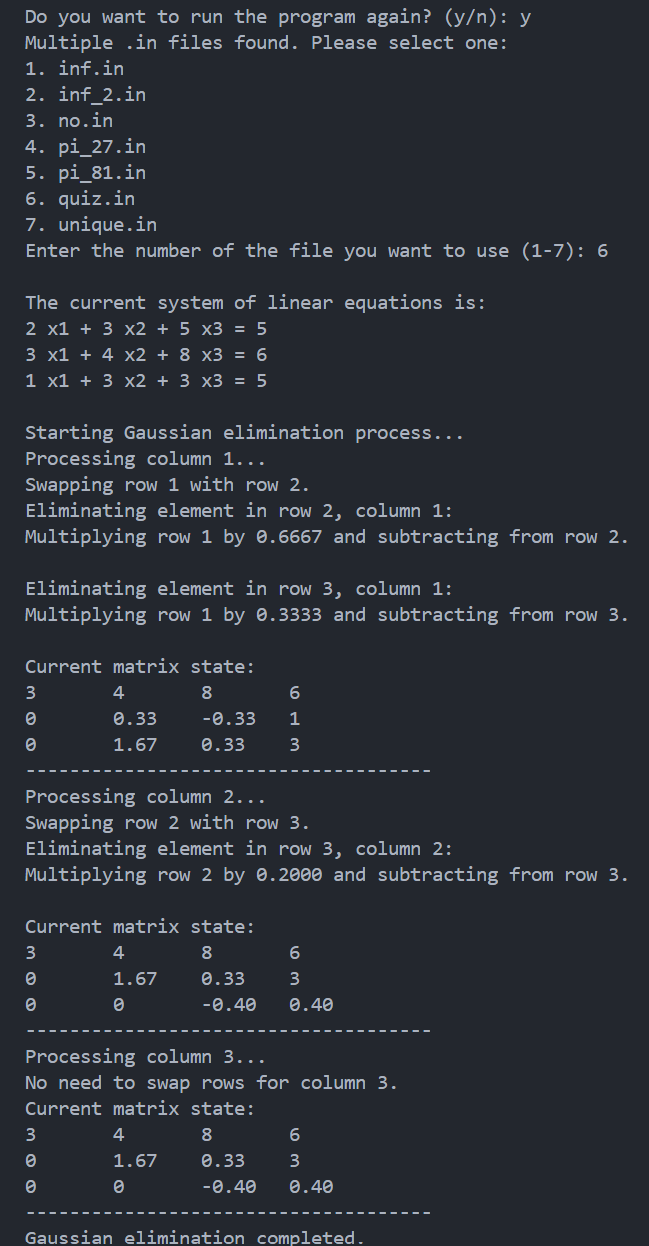
\includegraphics[width=0.4\textwidth]{Problem 2/figs/quiz_1.png}
	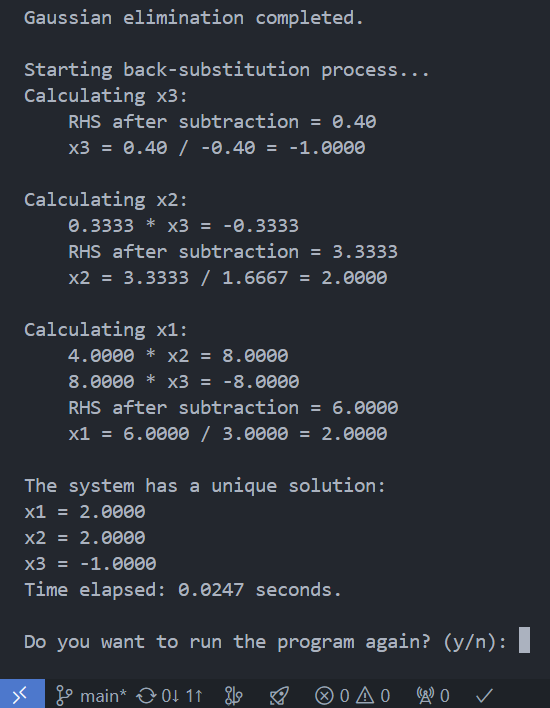
\includegraphics[width=0.5\textwidth]{Problem 2/figs/quiz_2.png}
	\caption{原题要求解的\texttt{quiz.in}}
\end{figure}

\begin{figure}[H]
	\centering
	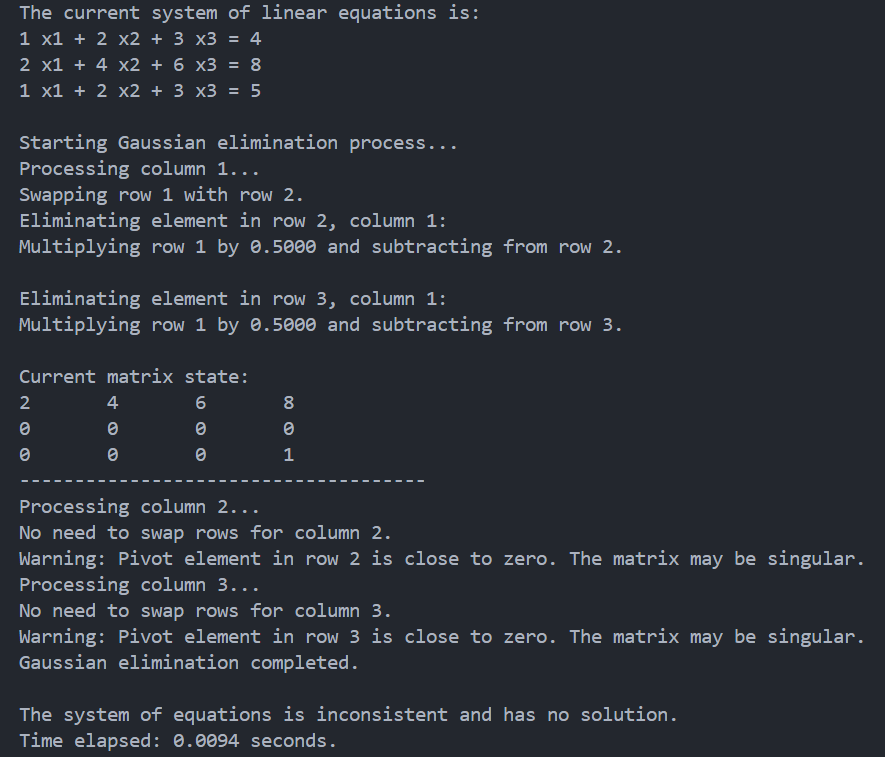
\includegraphics[width=1.0\textwidth]{Problem 2/figs/no.png}
	\caption{无解情形\texttt{no.in}}
\end{figure}

\begin{figure}[H]
	\centering
	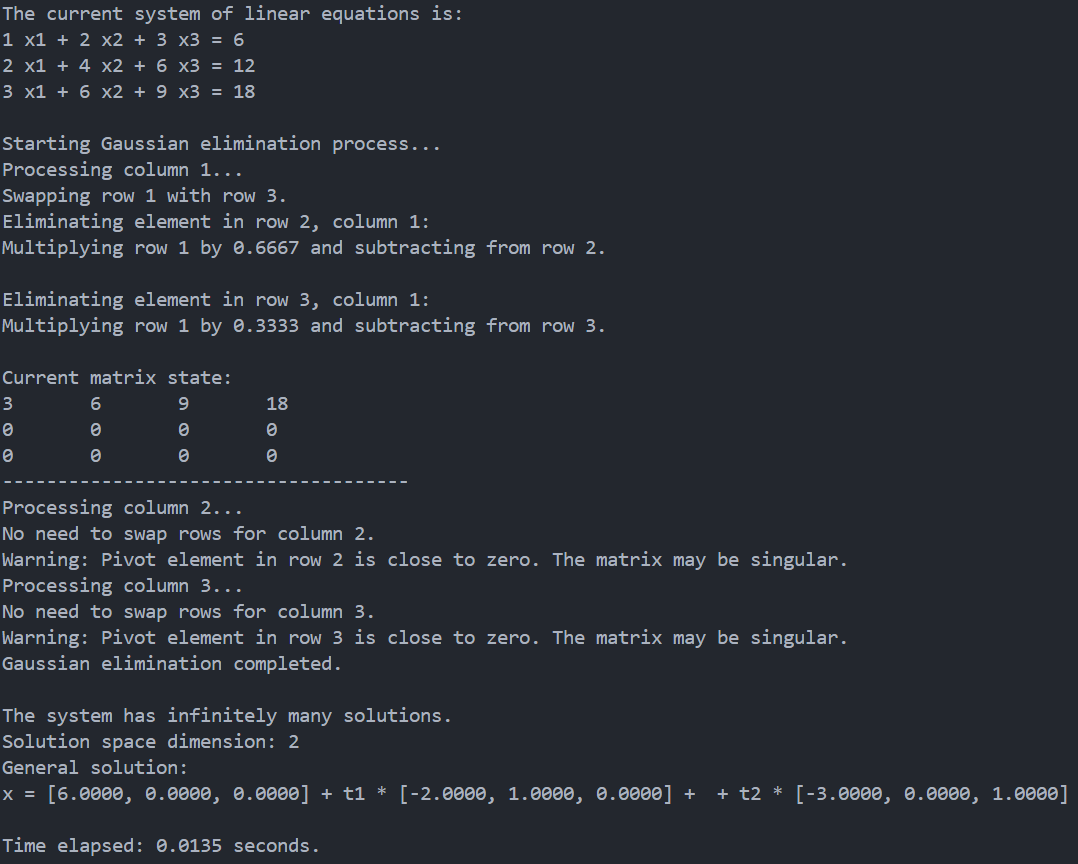
\includegraphics[width=0.75\textwidth]{Problem 2/figs/inf.png}
	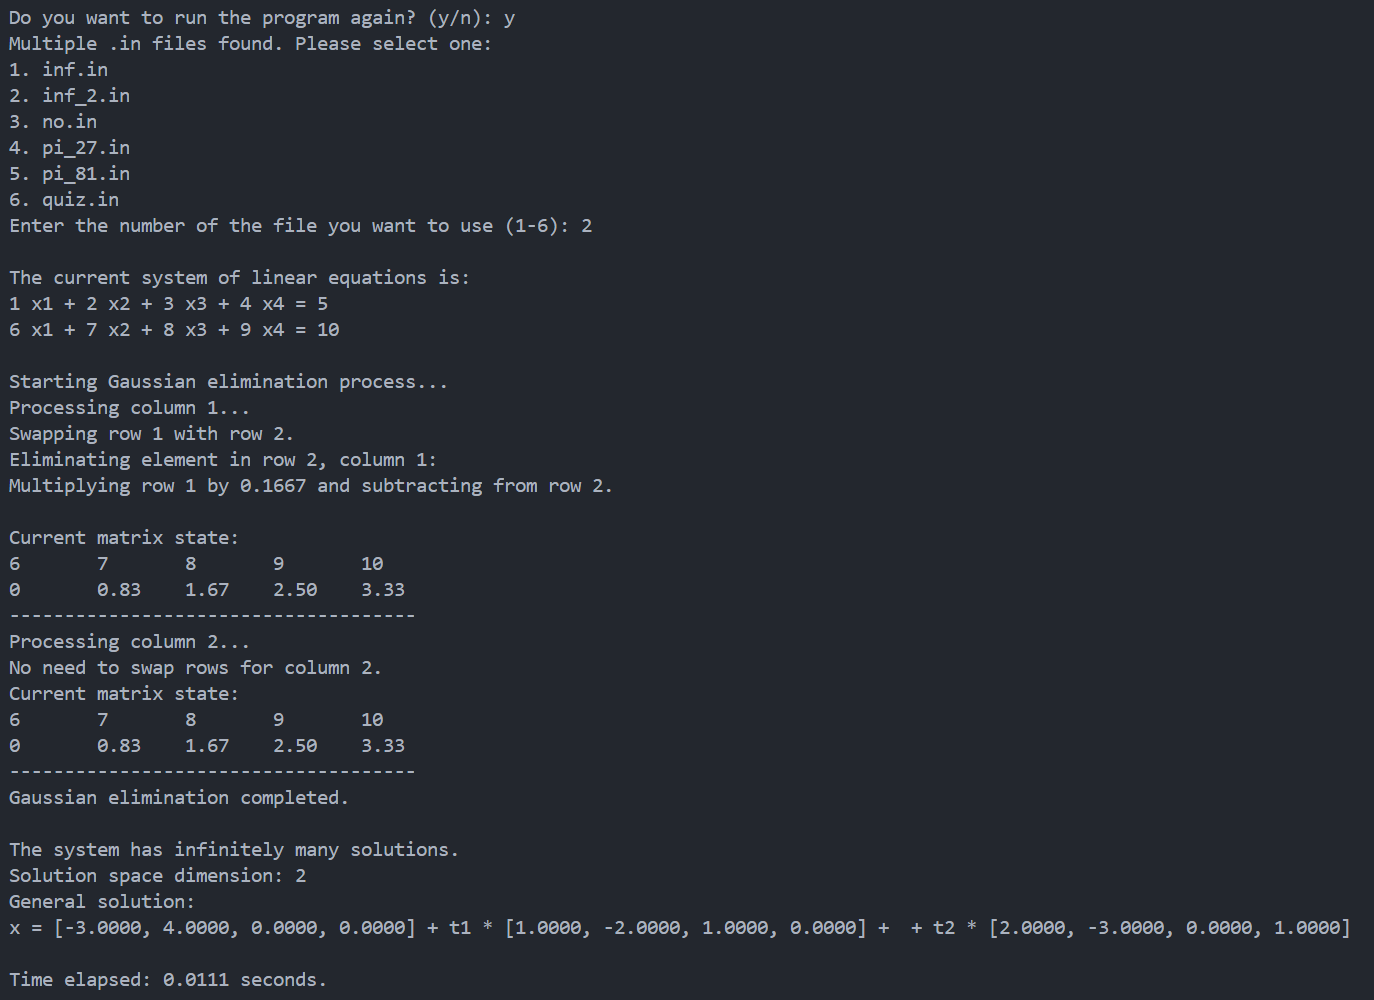
\includegraphics[width=0.75\textwidth]{Problem 2/figs/inf_2.png}
	\caption{两种无穷多组解情形\texttt{inf.in},\texttt{inf\_2.in}}
\end{figure}

\begin{figure}[H]
	\centering
	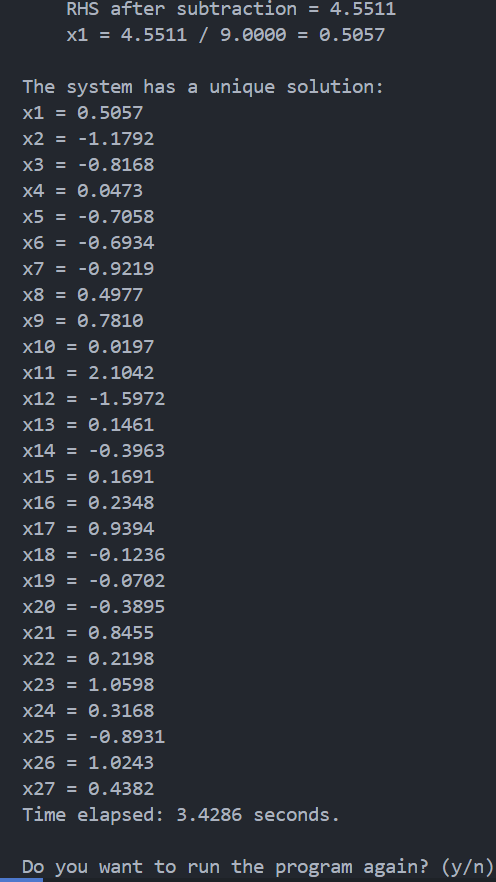
\includegraphics[width=0.3\textwidth]{Problem 2/figs/pi_27.png}
	\vspace{5pt}
	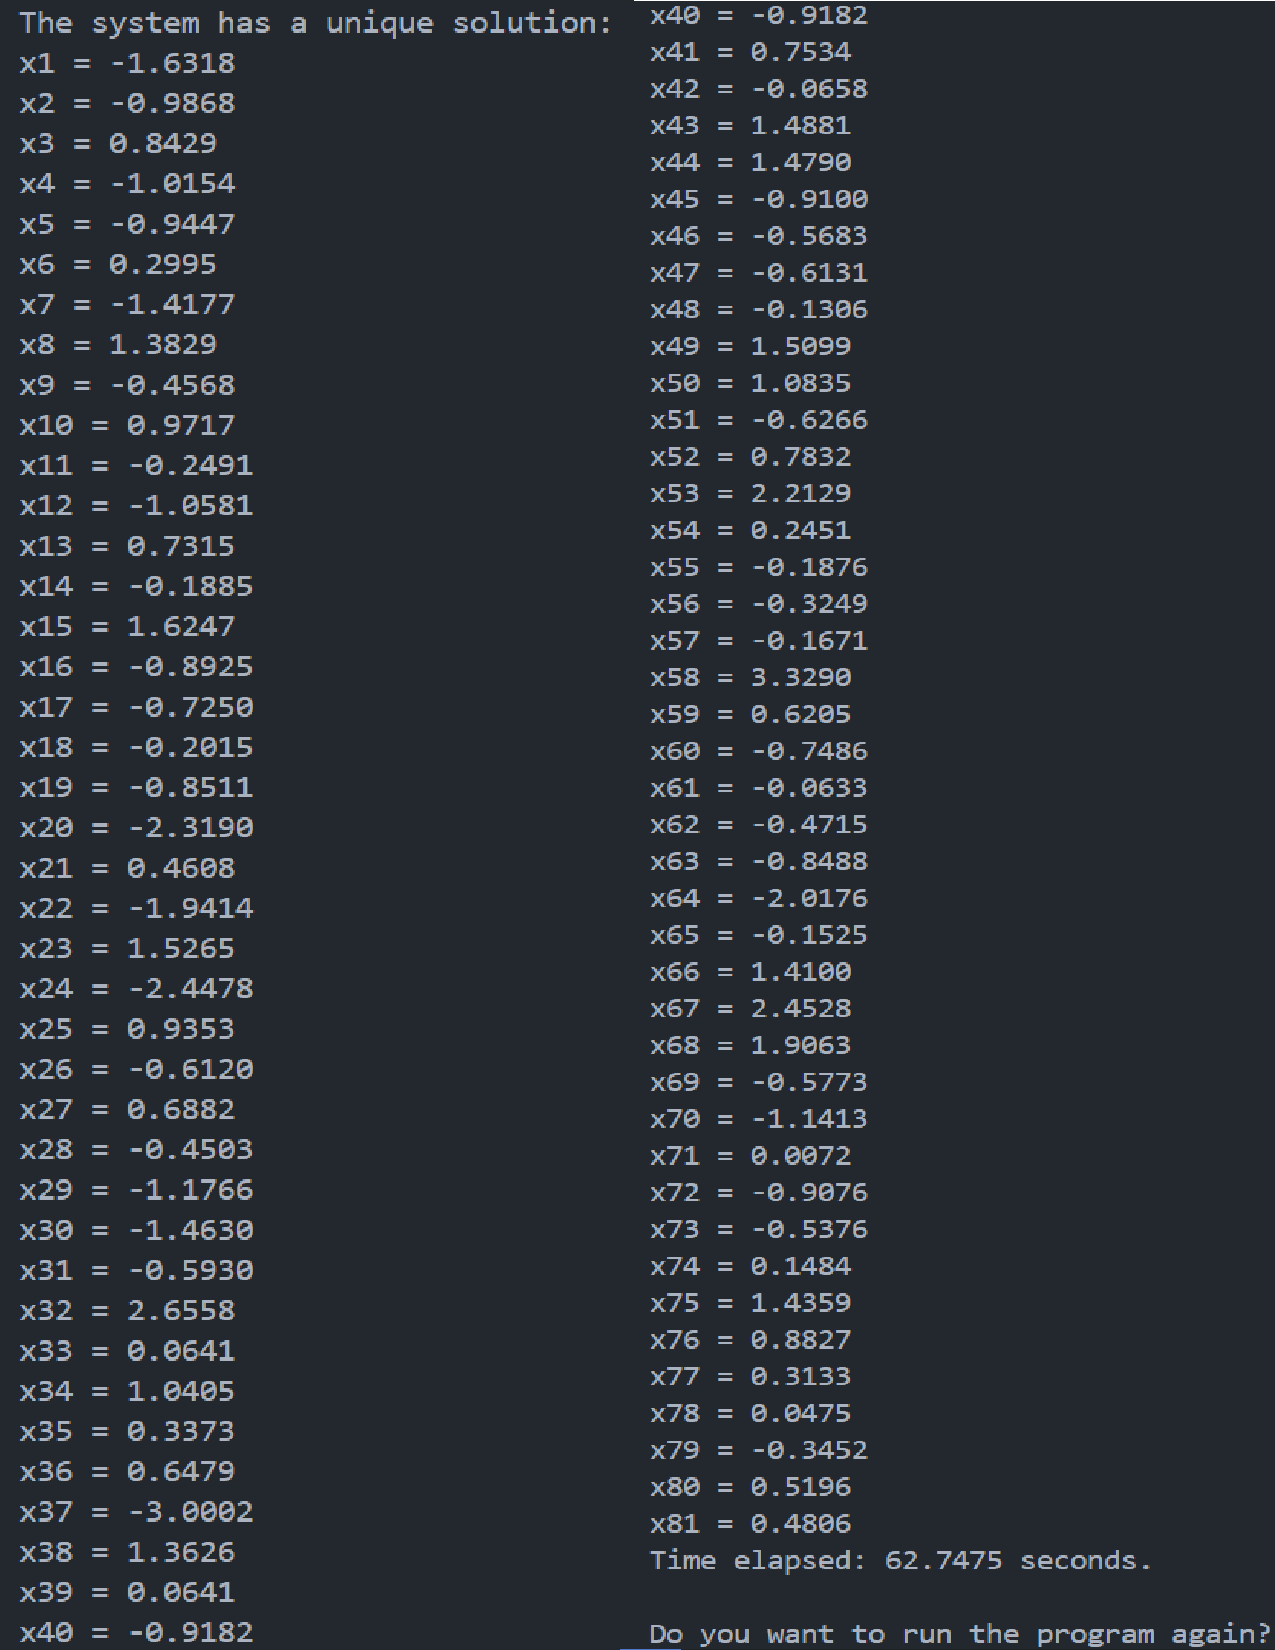
\includegraphics[width=0.6\textwidth]{Problem 2/figs/pi_81.pdf}
	\caption{圆周率提取的\texttt{pi\_27.in}和\texttt{pi\_81.in}对比}
\end{figure}

\begin{figure}[H]
	\centering
	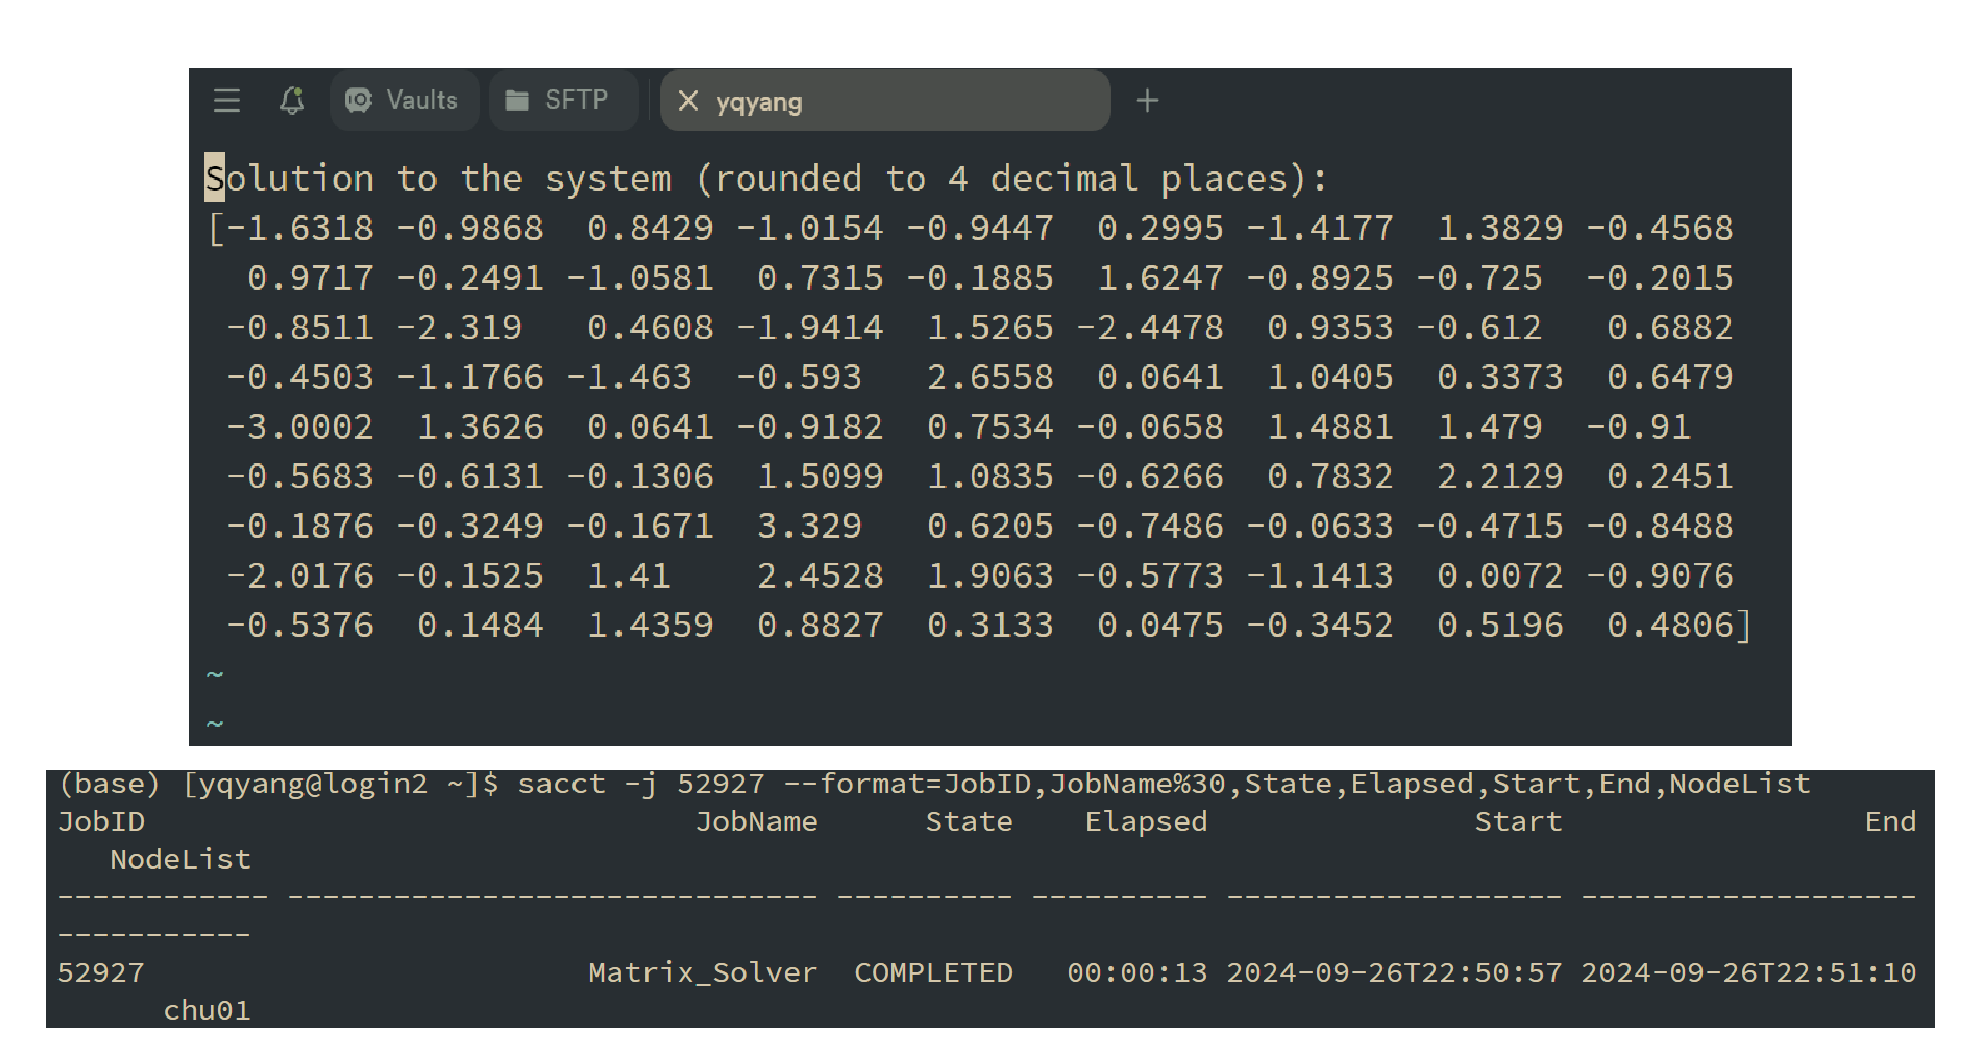
\includegraphics[width=1.0\textwidth]{Problem 2/figs/slurm.pdf}
	\caption{\texttt{pi\_81.in}使用\texttt{numpy}库求解的结果}
\end{figure}